% SEng 5852 - Spring 2013 White Paper Review
\documentclass{proc}
\usepackage{graphicx}
\setlength\parindent{0pt}

\title{
The GitHub Open Source Development Process
\author{Kevin Peterson\\
Department of Information Technology\\
Clinical Informatics Support Systems\\
Mayo Clinic\\
200 1st Street\\
Rochester, MN  55905\\
\small \texttt{peterson.kevin@mayo.edu}
}
}

\date{}

\begin{document}
\maketitle

\begin{abstract}
Open Source Software (OSS) has produced many successful projects. The development process by which these projects are produced is generally unstructured compared to commercial software -- but a definite pattern does arrive, and is no less a pattern. GitHub, a popular OSS code hosting website, and Git, the site's SCM of choice, may have the potential to fundamentally change ths process.\\
By analyzing a subset of GitHub repositories, this report will show how GitHub has influenced some very intrinsic aspects of traditional OSS develoment, such as developer hierarchies and issue close velicity. We find that... TODO
\end{abstract}

\noindent \textbf{Keywords.} Git, GitHub, OpenSource

\section{Introduction}
Open Source Software (OSS) has fundamentally changed how we view the Software Development Process\cite{raymond1999cathedral}. OSS projects are not only viable, but successful and thriving. 

A case study of the Apache Server project\cite{mockus2000case} shows that a dedicated community can produce software that rivals or exceeds commercial offerings. This study showed that even in the unstructured context of OSS, certain structures, hierarchies, and codes of conduct emerge. Contrast the Apache Server project to a successful project on GitHub. Although the spirit and intent may be the same, the tool set is drastially different. The intent of this paper is to explore how GitHub facilitates this process, and also how it may cause it to evolve.

\subsection{Hypothesis}
\emph{Hypothesis 1: As the number of Watchers increase, the number of Repository Forks will increase.}\\
In Open Source Software, a feeling of community belonging can be intrinsicly motivating to developers\cite{lakhani2003hackers}. This feeling of belonging can be expressed passively, as a \emph{watch}, or actively, as a \emph{fork} of a repository. As \emph{watches} don't necessarily signal intent to contribute, a positive direction for an OSS project is to not only increase the number of \emph{watchers}, but also the number of \emph{forks}. As both signify a general general interest in the project, it is expected that there be some correllation between the two.\\

\emph{Hypothesis 2: As the number Repository Forks increase, the Issue Resolution Time will decrease.}\\
In OSS, a project \emph{fork} has at times carried negative connotations, and has even been referred to as a hazzard\cite{kogut2001open}. In the context of Git and GitHub, however, a \emph{fork} is a positive occurence for a project, as it signifies greater project involvement. As Git allows for easy merging of \emph{forks}, code contributions in the form of defect fixes can be incorporated quickly. Because of this, it is expected that \emph{Issue Resolution Time} will decrease as the number of \emph{forks} increases.\\

The Apache Project noted that a rapid response to problems can be obtained because OSS is not bound to release schedules in the same way commercial software is. ``Patches'' may be released at any time, by any member of the community\cite{mockus2000case}. ``Patches"" in the context of GitHub could be equated to Pull Requests.\\

\emph{Hypothesis 3: There will be more Issue Reporters than Committers by an order of magnitude}\\
Research into the Apache Server project observed that there were far more \emph{Issue Reporters} than there were code \emph{Committers}\cite{mockus2000case}. The Apache Server project is an excellent case study in this type of Developer Hierarchy. Apache is built around a small set of {\it Core Developers}, followed by {\it Defect Repairers} and {\it Defect Reporters}. Each level of this hierarchy brings with it an order of magnitude increase in number of participants. The 10-15 {\it Core Developers} contribute around 80\% of the new functionality, while the rest of the 400 code contributors focus primarily on bug fixes. The {\it Defect Reporters} were by far the largest group, with over 3000 individuals submitting bug reports.\\

Because issue reporting is of low risk to the code base, but has potentially high value, it is a perfect way for large numbers of people to contribute. It is expected that the findings of the Apache Server project research will hold true for GitHub projects as well.\\

\subsection{Research Questions}

\emph{Research Question 1: Are GitHub projects primarily focused around a small set of core Committers?}\\
A smal core of developers, however, seems to be a historial fact of OSS development\cite{mockus2000case,mockus2000two,krishnamurthy2002cave}. At the extreme of this, a study of projects on the software hosting site Sourceforge\footnote{http://sourceforge.net} found that a large percentage of OSS development is done by lone developers. Is a small core of developers intrinsic to OSS development, or have the social aspects of GitHub and the distributed nature of Git changes this?

\emph{Research Question 2: What is the GitHub Philosophy?}\\
The socal aspects of GitHub are an important part of the experience\cite{dabbish2012social}. User interactions and social pressures can drive OSS development in interesting ways. Social aspects of OSS development have existed before GitHub, with mailing lists\cite{mockus2000case}, gift giving mechanisms\cite{bergquist2008power}, and other code hosting sites. What is GitHub doing to facilitate change on OSS development, and how does it see OSS development changing moving forward?

\emph{Research Question 3: Can GitHub be used for more that code artifacts?}\\
The Object Managment Group\textregistered\footnote{http://www.omg.org} computer industry consortium focused on technology standards. Potential standard summission teams must go through a vetting process\cite{kobryn1999uml} which allows industry representatives to provide feedback on the standard. Gathering and recording this feedback is a challenge, but GitHub's issue tracking system may be able to streamline the process.

\section{Methods}

\section{Results}
\subsection{Hypotheses}
\emph{Hypothesis 1: As the number of Watchers increase, the number of Repository Forks will increase.}\\
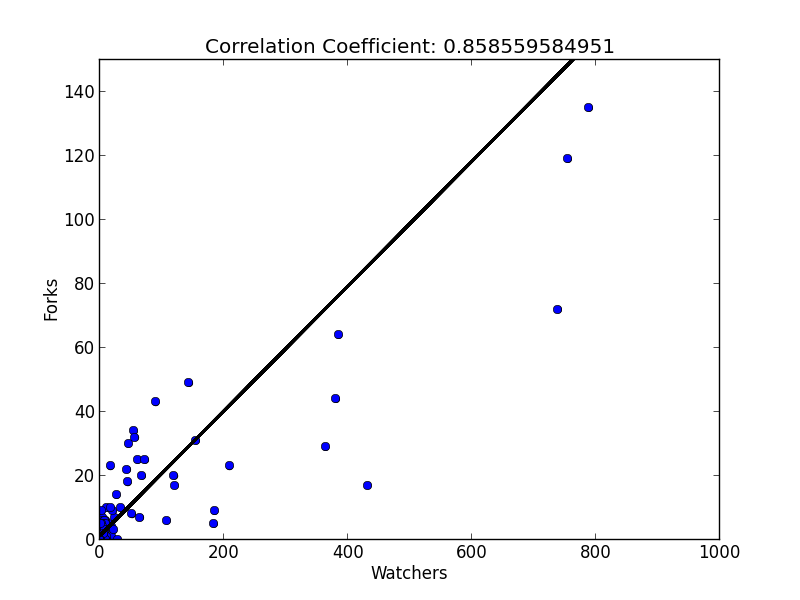
\includegraphics[height=3in,width=3in]{images/watcher_forks_scatterplot.png}

\emph{Hypothesis 2: As the number Repository Forks increase, the Issue Resolution Time will decrease.}\\
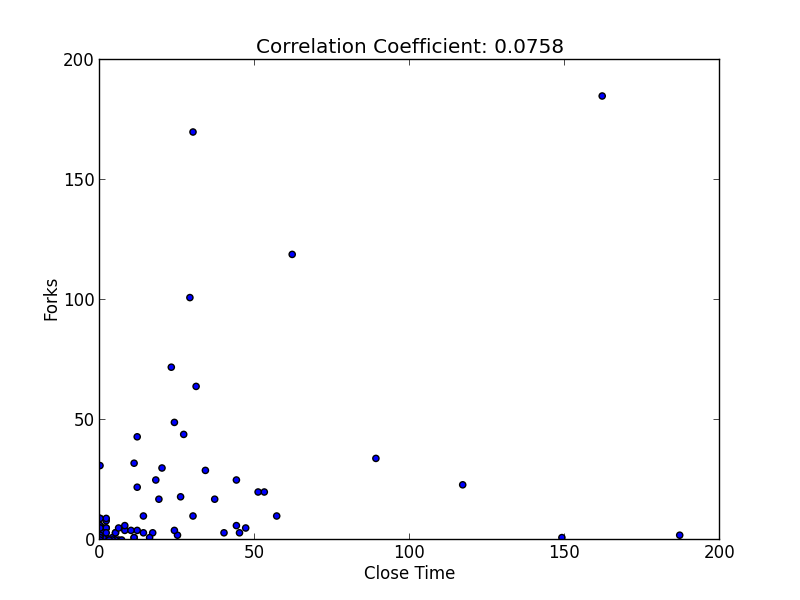
\includegraphics[height=3in,width=3in]{images/issue_close_time_forks_scatterplot.png}

\emph{Hypothesis 3: There will be more Issue Reporters than Committers by an order of magnitude.}\\
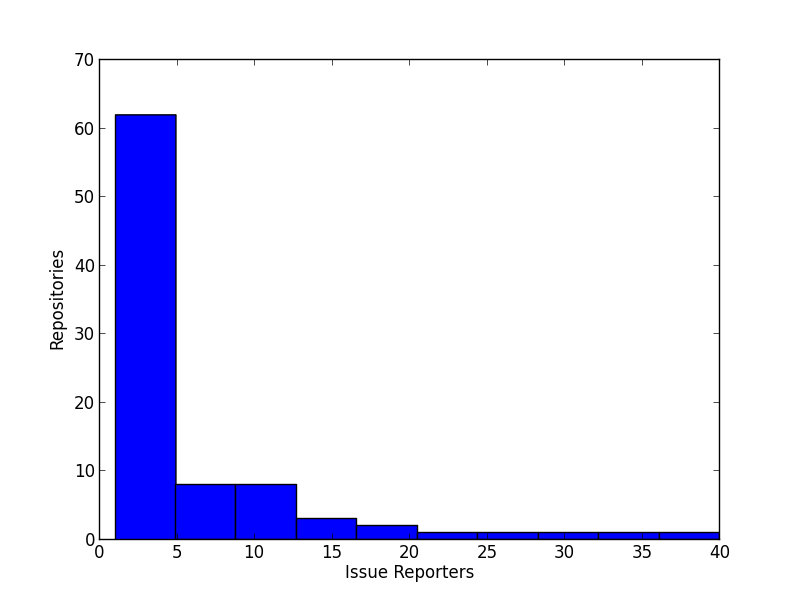
\includegraphics[height=3in,width=3in]{images/issue_reporters_histogram.png}
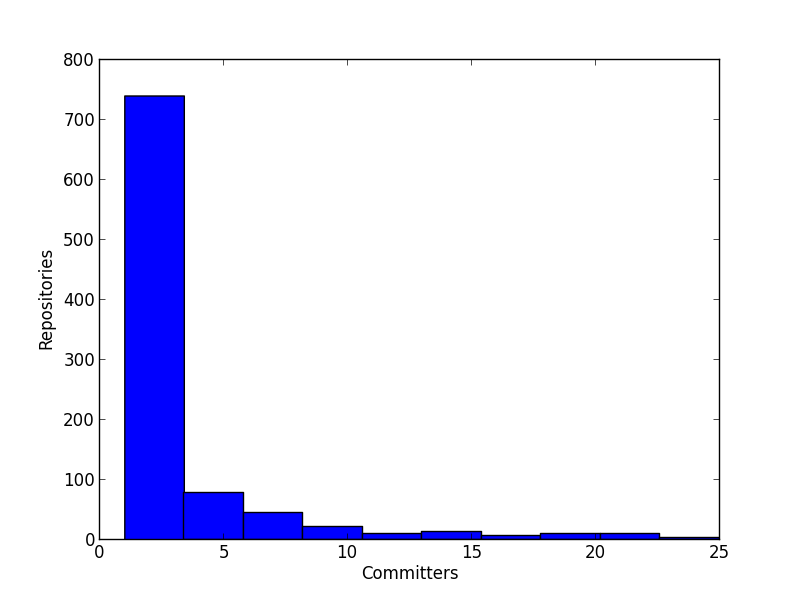
\includegraphics[height=3in,width=3in]{images/committers_histogram.png}
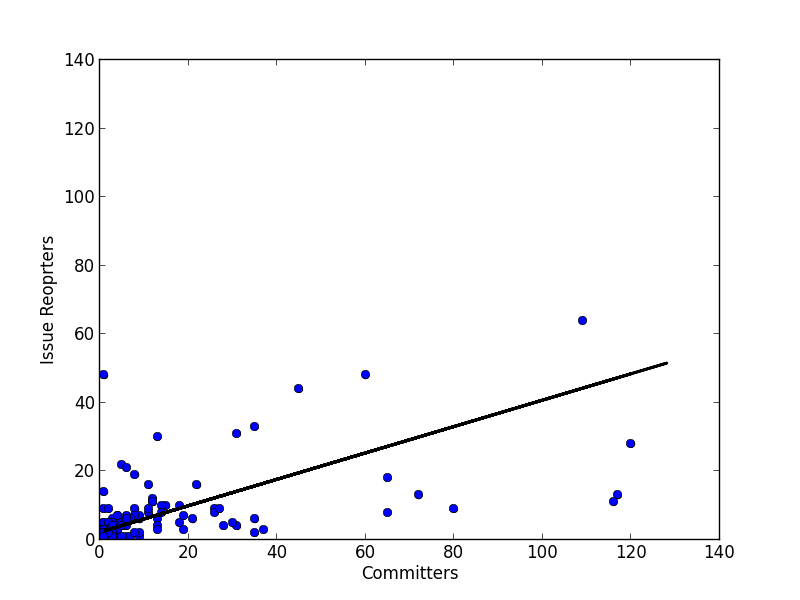
\includegraphics[height=3in,width=3in]{images/issue_reporters_committers_scatterplot.png}

\subsection{Research Questions}
\emph{Research Question 1: Are GitHub projects primarily focused around a small set of core Committers?}\\

\emph{Research Question 2: What is the GitHub Philosophy?}\\

\emph{Research Question 3: Can GitHub be used for more that code artifacts?}\\

\section{Acknowledgments}


  
\bibliographystyle{plain}
\bibliography{bibliography}




\end{document}
